\chapter{Features e Controlli}
 \section{Spiegazione}
 L'applicativo permette ad un utente dopo un login di cercare le risorse nella biblioteca online.
 La ricerce può avvenire sia tramite il nome della risorsa, sia tramite l'utilizzo di una serie di 
 filtri composti da delle Jcombobox.
 L'applicazione inoltre da la possibilità ad utente con permessi di amministratore di aggiundere risorse 
 al database.


 \subsection{Finestra di Login}
 Nella \textit{Finesta di Login} l'utente pu\'o decidere di effettuare un login per accedere all'applicativo, oppure,
 in caso non avesse un account, di registrarsi cliccando sulla scritta \textit{"Non hai un account? Clicca
 qui per registrarti"}.
 \\
 
\includegraphics[scale=0.25, center]{Immagini/Schermate/Login_Register/LoginPage.png}

 \subsection{Finestra di Registrazione Utente}
 Nella \textit{Finestra di Registrazione} l'utente deve riempire i campi "Username", "Password", "Conferma Password" per creare un
 nuovo account. Qualora un account con quello Username dovesse gi\'a esistere, oppure le due Password non dovessero
 essere uguali, l'appilcativo segnaler\'a l'errore e colorer\'a il bordo dei Jtextfield di rosso.
 \\
 
\includegraphics[scale=0.25, center]{Immagini/Schermate/Login_Register/RegisterPage.png}

 \subsection{Finestra di Ricerca}
 Nella \textit{Finesta di Ricerca} sar\'a possibile cercare una risorsa nel database inserendone il titolo nel Jtextfield e 
 selezionandone il tipo. Nel caso in cui l'utente non conoscesse il titolo del libro potrà usare la sezione filri che cambia 
 in base al tipo di risorsa selezonata.
 La sezione filtri è composta da dei Jcombobox attivabili tramite Jcheckbox differenti in base alla risorsa da ritrovare.
 \\
 
\includegraphics[scale=0.25, center]{Immagini/Schermate/Search/SearchPage.png}

 \subsubsection{Filtri Libri}
 
\includegraphics[scale=0.25, center]{Immagini/Schermate/Search/SearchPage-FiltriLibro.png}
 \subsubsection{Filtri Serie}
 
\includegraphics[scale=0.25, center]{Immagini/Schermate/Search/SearchPage-FiltriSerie.png}
 \subsubsection{Filtri Articoli}
 
\includegraphics[scale=0.25, center]{Immagini/Schermate/Search/SearchPage-FiltriArticoli.png}
 \subsubsection{Filtri Riviste}
 
\includegraphics[scale=0.25, center]{Immagini/Schermate/Search/SearchPage-FiltriRiviste.png}

 \subsection{Finestra dei Risultati}
 Nella \textit{Finestra dei Risultati} è possibile trovare una JTable con tutti i risultati della query
 \\
 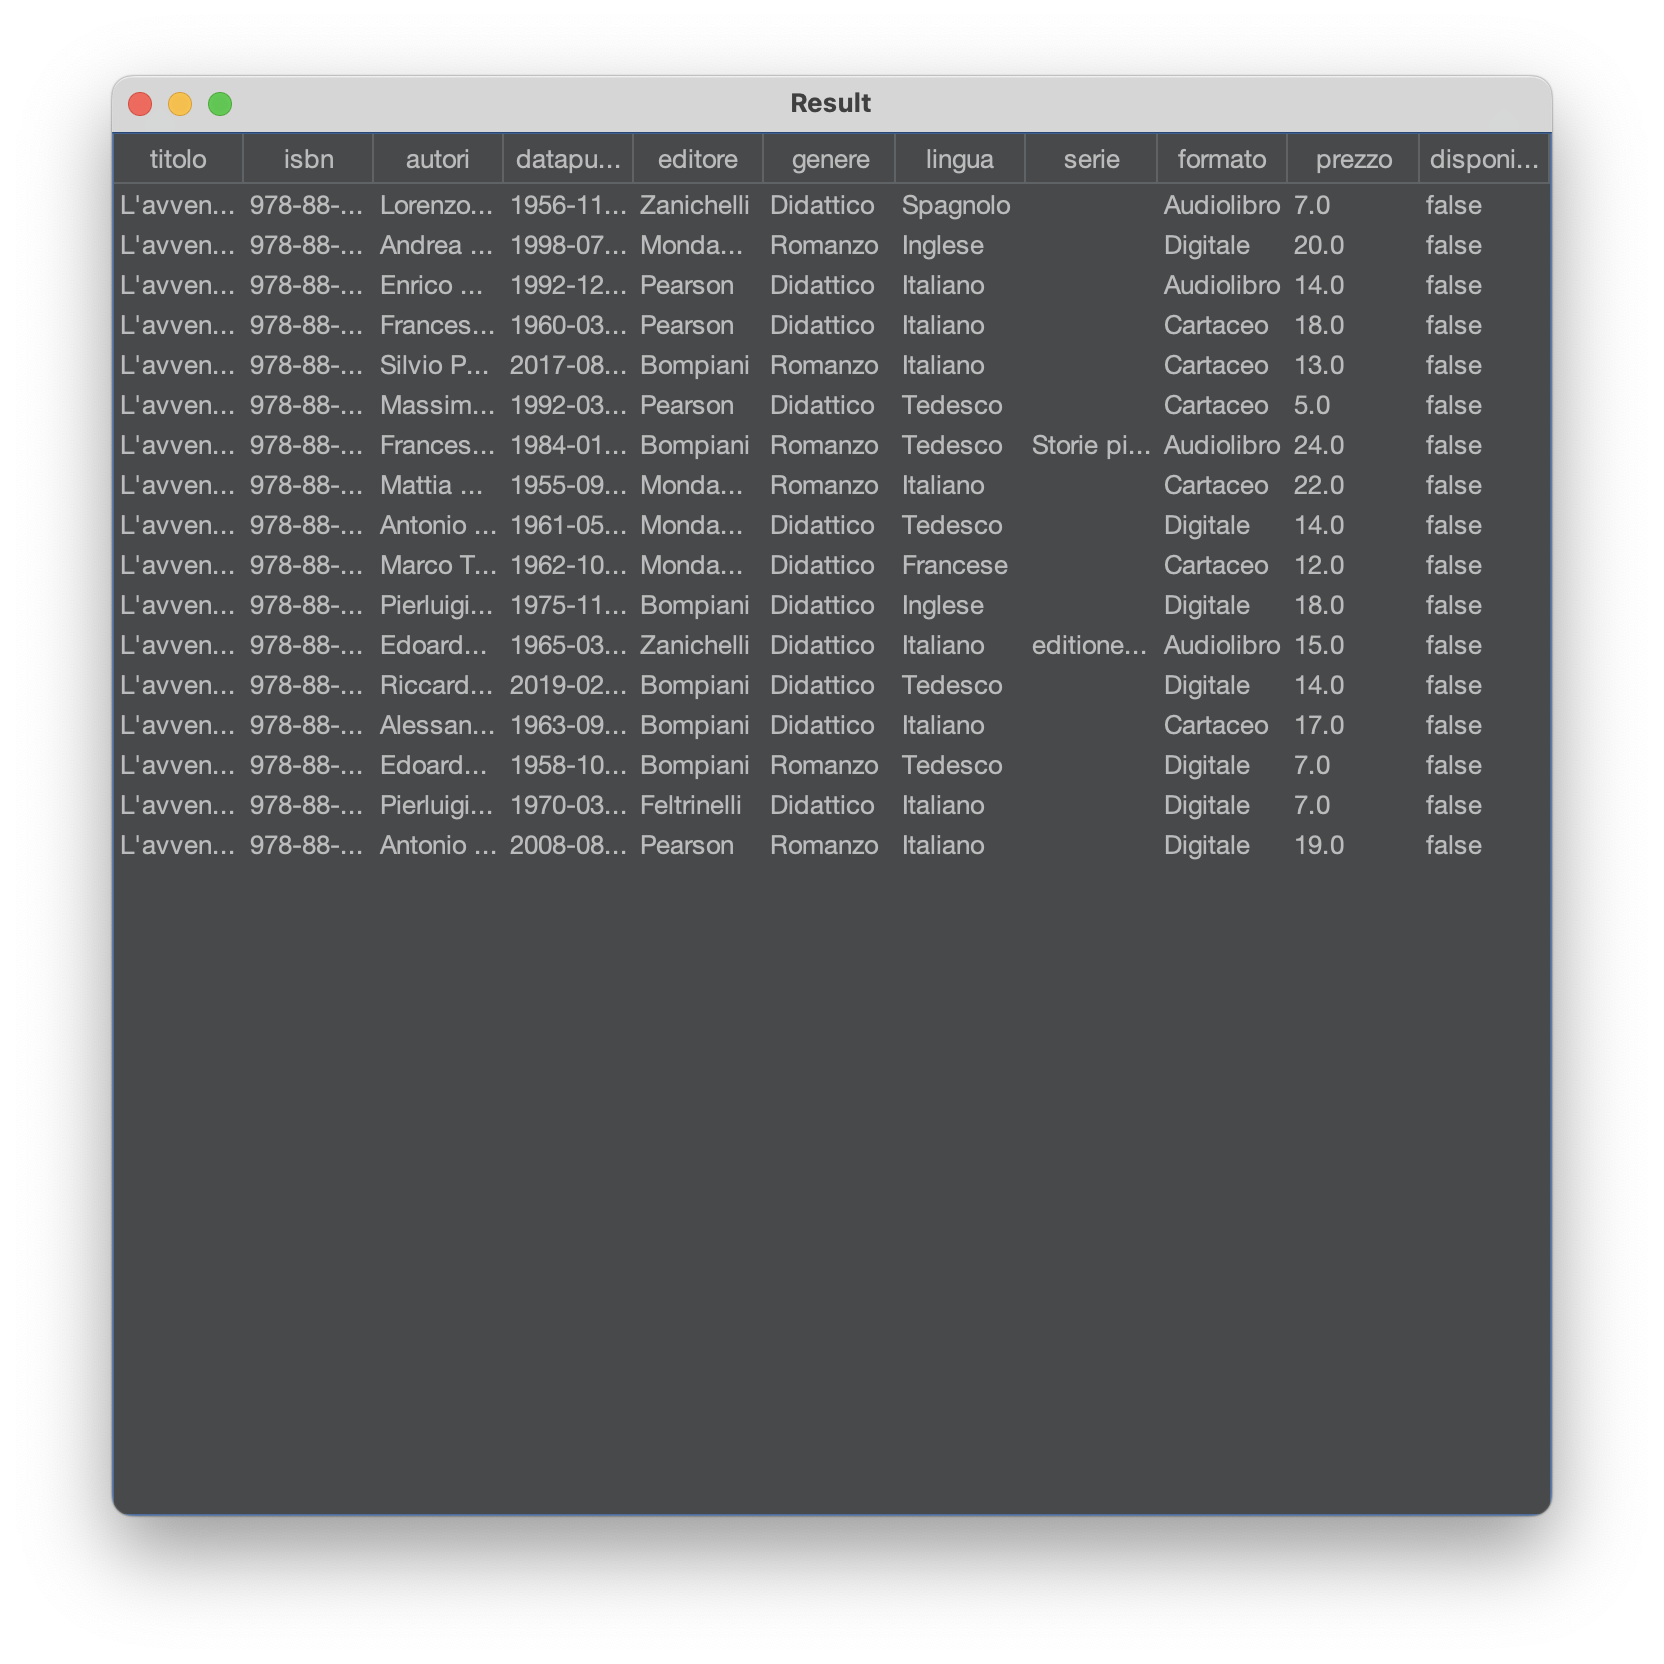
\includegraphics[scale=0.25, center]{Immagini/Schermate/Search/ResultPage.png}

 \subsection{InsertPage}
 Nella \textit{Finestra di Inserimento} è p
 
\includegraphics[scale=0.25, center]{Immagini/Schermate/Insert/InserisciRisorsaPage.png}

 \subsubsection{Libro}
 
\includegraphics[scale=0.25, center]{Immagini/Schermate/Insert/InserisciRisorsaPage-Libro.png}
 \subsubsection{Libro in Serie}
 
\includegraphics[scale=0.25, center]{Immagini/Schermate/Insert/InserisciRisorsaPage-LibroSerie.png}

 \subsubsection{Articolo}
 
\includegraphics[scale=0.25, center]{Immagini/Schermate/Insert/InserisciRisorsaPage-Articolo.png}
 \subsubsection{Articolo in Rivista}
 
\includegraphics[scale=0.25, center]{Immagini/Schermate/Insert/InserisciRisorsaPage-ArticoloRivista.png}
 \subsubsection{Articolo in Conferenza}
 
\includegraphics[scale=0.25, center]{Immagini/Schermate/Insert/InserisciRisorsaPage-ArticoliConferenza.png}

 \subsection{Utente}
 \subsubsection{Notifiche}
 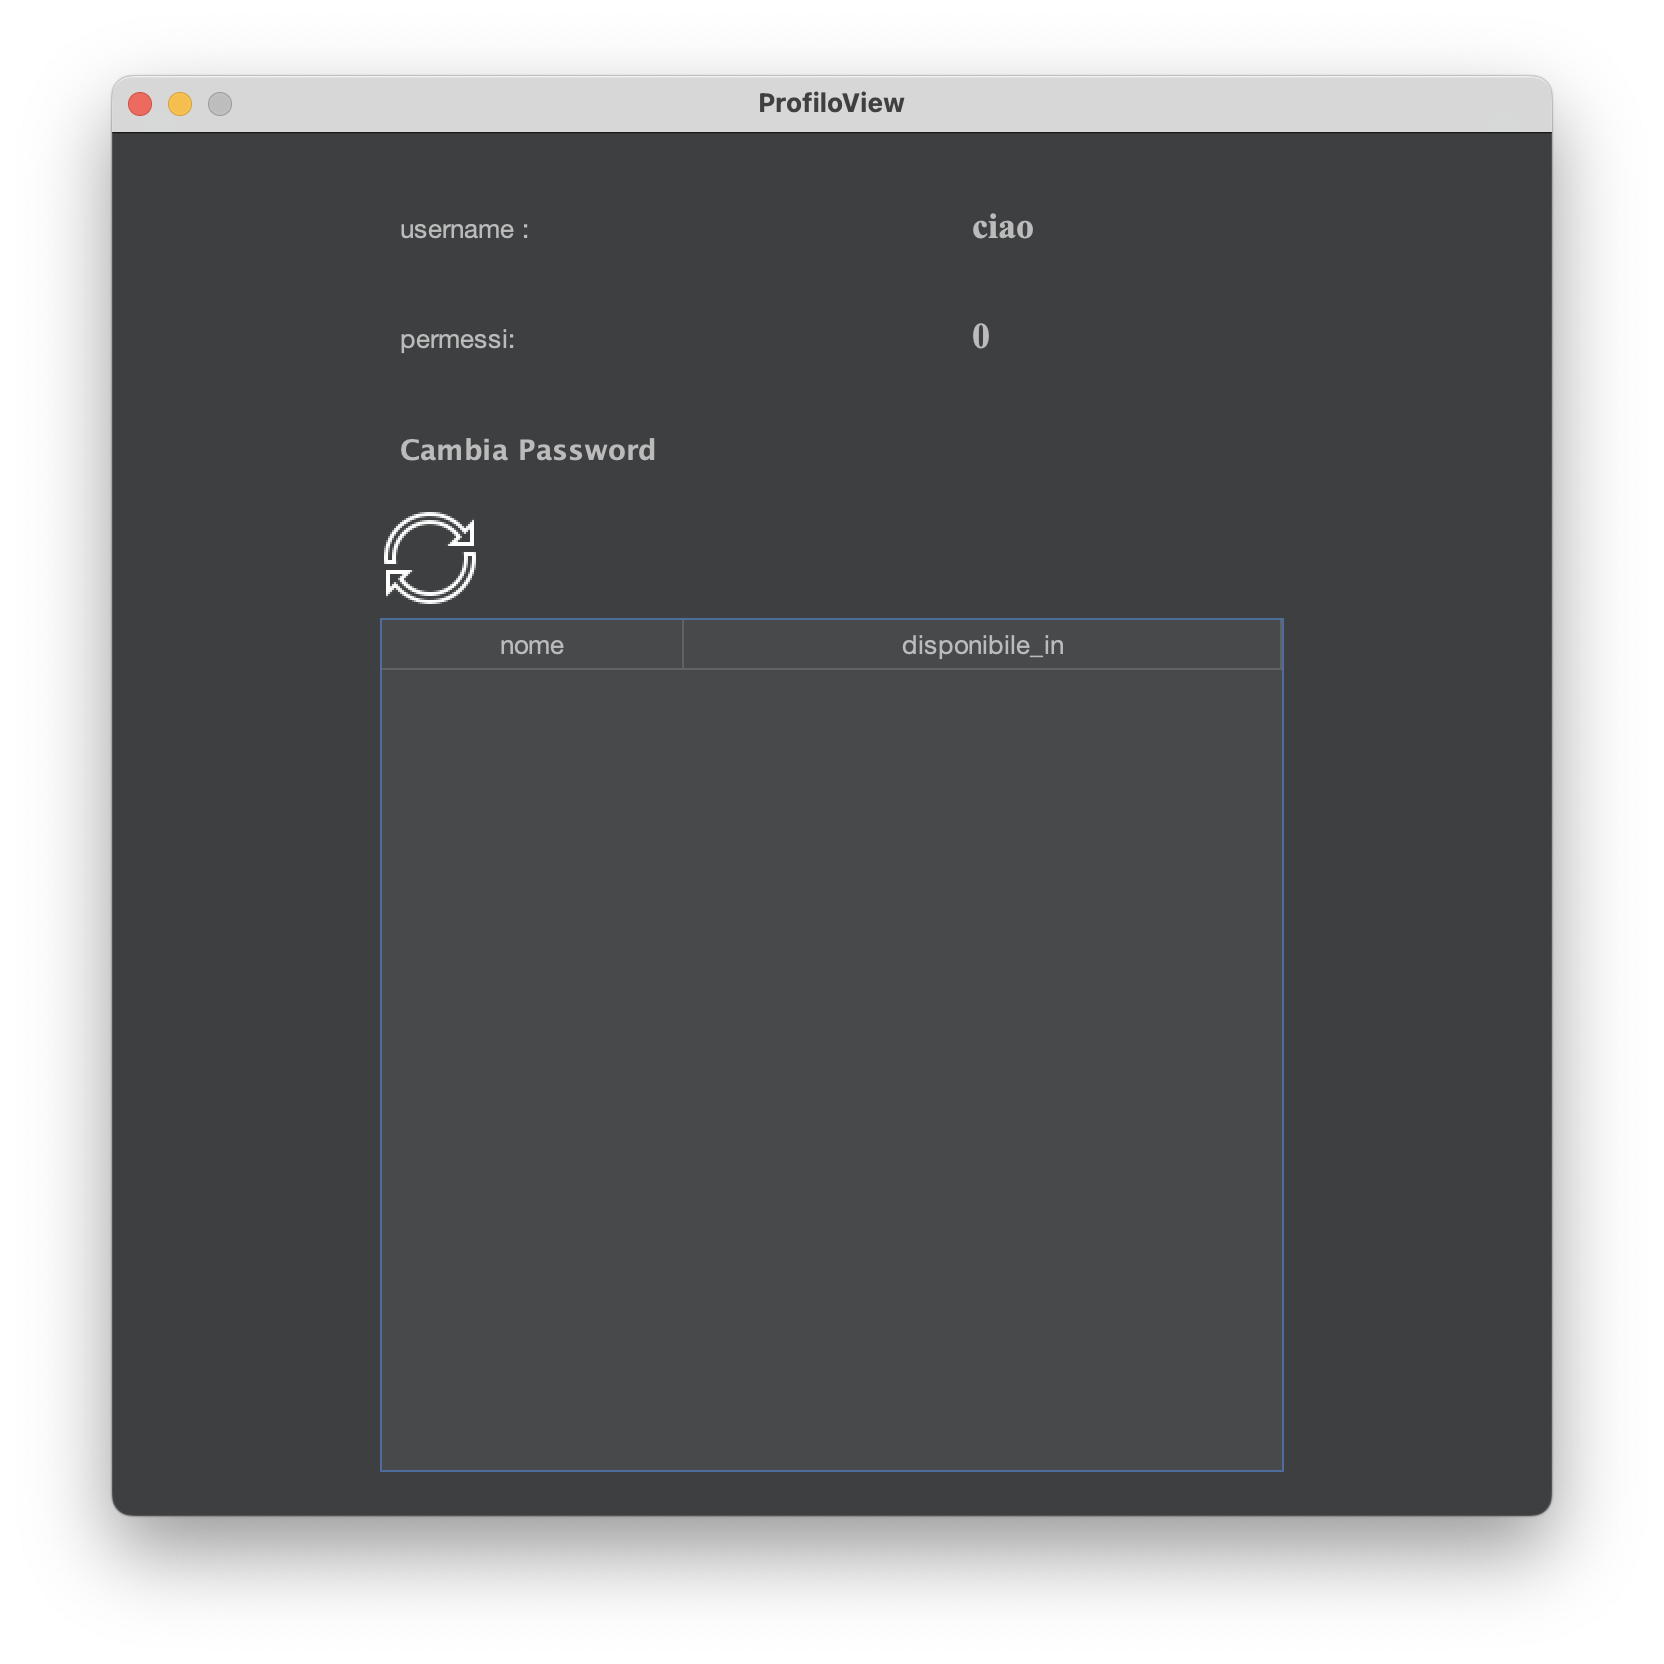
\includegraphics[scale=0.25, center]{Immagini/Schermate/Utente/NotificheUtente.png}
 \subsubsection{Richiesta di disponibilit\'a Serie}
 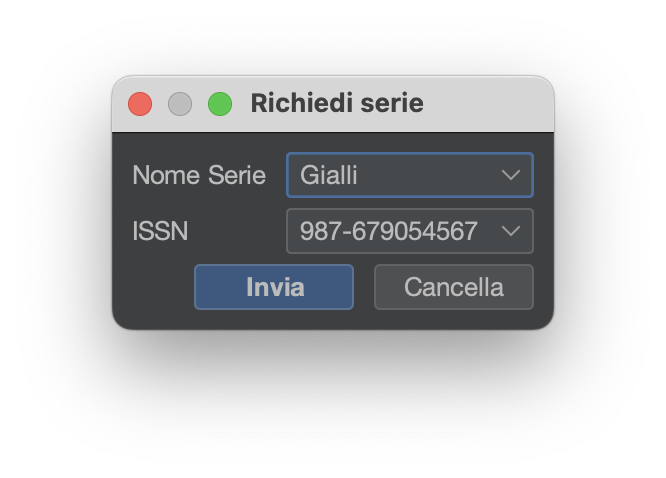
\includegraphics[scale=0.50, center]{Immagini/Schermate/Utente/RichiediDisponibilita.png}